\subsection{Alternative model "Globally Ordered Data" (GOD)}


% \tm {Laisser présentation du modèle, graphical model, estimation des paramètres. Tous les lemmes et théorèmes vont en annexe.}

In the article under study, the authors motivated the use of binary search with the following sentence: "In order to minimize the number of potentially wrong comparisons, it
is necessary to minimize the number of comparisons performed during the search process.". However, we believe that minimizing the number of incorrect comparisons may not be an adequate intuition, and it is more crucial to minimize the probability of making a wrong guess. Motivated by this perspective, we have developed an alternative model where the data is compared with each category with some noise. We will refer to this model as the Globally Ordered Data (GOD) model.

We still consider a search for the parameter $\mu$ among the ordered categories. However, instead of conducting a binary search, we compare each category to the parameter $\mu$ and with probability $\pi$ we get the correct answer. After making all these comparisons, we then select the category that corresponds to the minimum number of comparison error. This approach display similar properties to the BOS model such as a unique mode, probability distribution decrease on either side of the mode, and the flexibility to accommodate uniform or Dirac distribution.

\subsubsection{Probabilistic model}

\begin{figure}[htbp]
    \centering
    \begin{tikzpicture}
     \node[obs]                               (xj) {$x_i$};
     \node[latent, left=1.4cm of xj]               (cj) {$C[j]$};
     \node[latent, left=of cj]               (zj) {$Z_j$};
     \node[const, left=of zj]    (pi) {$\pi$};
     \node[const, above=of cj]  (mu) {$\mu$};
    
     \edge{zj}{cj};
     \edge{cj}{xj};
     \edge {mu} {cj};
     \edge {pi} {zj};
    
     \plate[inner sep=.55cm] {}{(xj)(cj)(zj)}{$i=1, \ldots, n$};
     \plate[inner sep=.25cm] {}{(cj)(zj)}{$j=1, \ldots, m - 1$};
    \end{tikzpicture}
    \caption{Graphical model of the GOD model.}
    \label{fig:god_graphical_model}
\end{figure}
    
The GOD model for $m$ categories is characterized by two parameters $\mu \in \bbrack{1, m}, \pi \in ]\frac{1}{2}, 1]$. The observed data is only the selected category $x$. The latent variables are the vector $Z = (Z_1,...,Z_{m-1}) \in \set{0, 1}^{m - 1}$ and $C \in \set{0, 1}^{m-1}$.
$(Z_j)_{j\in\bbrack{1,m-1}}$ is a vector of independent Bernoulli variables, with parameter $\pi$. For $j \in \bbrack{1, m-1}$, $Z_j$ indicates whether the comparison with the category $j$ is correct $(Z_j=1)$ or not $(Z_j=0)$. $C$ is the vector containing the $m$ results of the comparisons depending on both $Z$ and the parameter $\mu$. It is defined as follows:
\[
\forall j \in \bbrack{1, m-1}, C[j] = \begin{cases}
    (\mu < j) & \text{if}\  Z_j = 1\\
    (\mu \not< j) & \text{if}\  Z_j = 0
\end{cases} \]

The GOD model will generate $x \in \bbrack{1, m}$ such that $x \sim \mathcal{U}(\argmin_{k \in \bbrack{1, m}} \norm{c - E_k}_1)$. We can interpret this as a probability maximization as stated in Theorem~\ref{thm:projection}. The graphical model associated with this probabilistic model is depicted on Figure \ref{fig:god_graphical_model}.


\begin{definition}[Heaviside vector]
    For $k \in \bbrack{1, m}$, we define:
    \[E_k := (1)^{k-1} (0)^{m - k} = (\underset{k-1}{\underbrace{1, \dots, 1}}, \underset{m - k}{\underbrace{0, \dots, 0}} ). \]
\end{definition}


\begin{thm}
    \label{thm:projection}
    If we suppose that the prior distribution of $\mu$ is uniform over $\bbrack{1, m}$ and $\pi > \frac{1}{2}$, then \(\forall c \in \set{0, 1}^{m-1}\),
    \[\argmax_{k \in \bbrack{1, m}} \Pr(\mu = k | C = c) = \argmin_{k \in \bbrack{1, m}} \norm{c - E_k}_1.\]
\end{thm}

The proof can be found in appendix~\ref{thm:projection_appendix}.

\subsubsection{Parameter estimation}

We want to estimate $\pi$ and $\mu$ from a sample $X = (x^1, \dots, x^n) \in \bbrack{1, m}^n$ of $n$ observations of $x$ generated by the GOD model. We aim at maximizing the likelihood of the sample : $\Pr(X | \pi, \mu)$. 

We define for $x \in \bbrack{1, m}$, 
\[ \mathcal{C}_x := \set{c \in \set{0, 1}^{m-1} | x \in \argmin_{k \in \bbrack{1, m}} \norm{c - E_k}_1 } .\]

\begin{lemma}
    \label{lemma:p_x_c_knowing_pi_mu}
    \[\Pr(x, c | \pi, \mu) = \indic{}_{\mathcal{C}_x}(c) \frac{\pi^{m - 1 - \norm{c - E_{\mu}}_1} (1 - \pi)^{\norm{c - E_{\mu}}_1}}{\card{\argmin_{k \in \bbrack{1, m}} \norm{c - E_k}_1}} .\]
\end{lemma}

Proof in appendix~\ref{lemma:p_x_c_knowing_pi_mu_appendix}.


\begin{definition}
    We define for $x \in \bbrack{1, m}, \mu \in \bbrack{1, m}, d \in \bbrack{0, m-1}$:
    \[ u(x, \mu, d) := \sum_{c \in \mathcal{C}_x / \norm{c - E_{\mu}}_1 = d}  \card{\argmin_{k \in \bbrack{1, m}} \norm{c - E_k}_1}^{-1} .\]
\end{definition}

For a given $m$, $u$ can be fully computed in $\mathcal O(m^2 2^m)$ time. We believe that it might be possible to compute it in polynomial time, but we did not have time to find how. Although still costly, it only needs to be computed once for a given $m$ and can be stored in $\mathcal O(m^3)$ space.
% copilot :
% Indeed, for a given $x$ and $\mu$, we have $\card{\mathcal{C}_x} = \binom{m}{\mu}$ and $\card% {\argmin_{k \in \bbrack{1, m}} \norm{c - E_k}_1} = \binom{m}{\mu - d} \binom{m - \mu + d}{d}$. Therefore, we have:

\begin{definition}[weighted likelihood]
    For the AECM algorithm, we define the weighted likelihood with weights $w \in \RR_+^n$:
    \[ \Pr((X, W') | \pi, \mu) = \prod_{i=1}^{n} \Pr(x^i | \pi, \mu)^{w'_i} \]

    As  $X \in \bbrack{1, m}^n$, without loss of generality, we can assume that we have exactly $m$ weights: $W = (\sum_{i / x^i = 1} W'[i], \dots, \sum_{i / x^i = m} W'[i])$. Hence with $W \in \RR_+^m$:
    \[ \Pr((X, W') | \pi, \mu) = \Pr(W | \pi, \mu) = \prod_{i=1}^{m} \Pr(i | \pi, \mu)^{w_i} \]

    And again, without loss of generality, we can assume that every sample is weighted with weight $w'_i = 1$.

    Hence we now consider data as a vector $W \in \RR_+^m$.
\end{definition}

\begin{thm}[Data likelihood]
    \label{thm:p_xs_knowing_pi_mu}
    \begin{align}
        \Pr(W | \pi, \mu) 
        &= \pi^{(m-1)\sum_{i=1}^{m} w_i} \prod_{i=1}^{m} \left[\sum_{d = 0}^{m-1} \left(\frac{1 - \pi}{\pi}\right)^d u(x^i, \mu, d) \right]^{w_i}\\
        L_W(\pi, \mu) 
        &= (m-1)\left(\sum_{i=1}^{m} w_i\right) \log\pi + \sum_{i=1}^{m} w_i \log\left[ \sum_{d = 0}^{m-1} \left(\frac{1 - \pi}{\pi}\right)^d u(x^i, \mu, d) \right]
    \end{align}
\end{thm}
\begin{proof}
    We just use the fact that the random variables $(x^i)_{i=1}^n$ are independent and Theorem~\ref{thm:p_x_knowing_pi_mu} from Appendix~\ref{appendix:god}.
\end{proof}

Similarly to the BOS model, we estimate $\hat{\pi}$ for each fixed $\mu$. Then we keep the couple $(\hat{\pi}, \mu)$ that maximizes the log-likelihood.
To estimate $\pi$ for a fixed $\mu$, we considered different possibilities. The first option is to use a simple grid search. This is feasible as evaluating $L_X$ is not too costly and can be done in $\mathcal O(nm)$ time. Then, we considered using the EM algorithm, similar to the approach taken for the BOS model. We derived the update rules and implemented it. Unfortunately, there was an issue with our EM implementation for this model that we did not succeed in fixing.

\begin{figure}
    \centering
    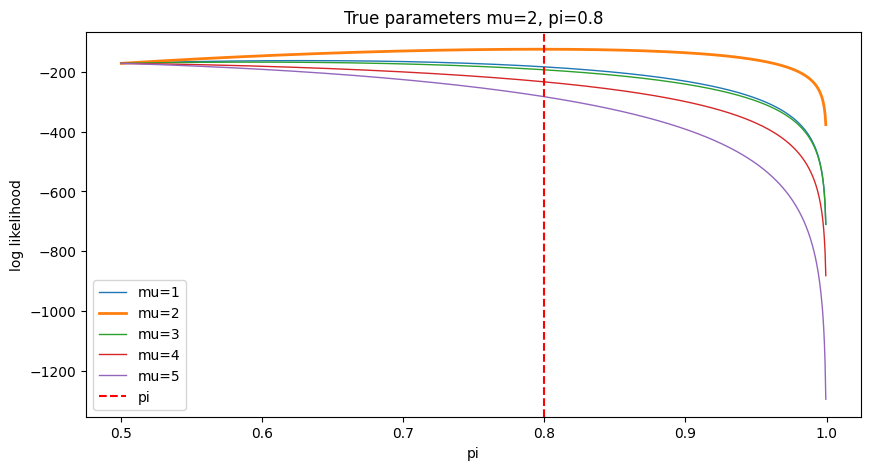
\includegraphics[width=0.5\textwidth]{Attachments/log_likelihoods.png}
    \caption{Log-likelihoods for each possible $\mu$ for $n = 100$ samples with the true parameters being $m = 5$, $\mu=2$ and $\pi = 0.8$ }
    \label{fig:log_likelihoods}
\end{figure}

We can examine the log-likelihood functions in Figure~\ref{fig:log_likelihoods} to understand how to optimize them. As observed, each of the functions $\pi \mapsto L_X(\pi, \mu)$ is concave on the interval $[0.5, 1]$.

\begin{thm}
    \label{thm:log_likelihood_concave}
    $\forall \mu \in \bbrack{1, m}$, 
    \[ \pi \mapsto L_W(\pi, \mu) \]
    is concave on $[0.5, 1]$.
\end{thm}

For the proof, see appendix~\ref{thm:log_likelihood_concave_appendix}.

As the log-likelihood is concave, we can employ the trichotomy method to find the maximum with a few evaluations of $L_W$. For a precision $\epsilon$, the trichotomy method requires $k \geq \frac{\lg_2 \epsilon + 1}{1 - \lg_2 3} = \mathcal O(\ln \epsilon)$ steps and therefore $\mathcal O(\ln \epsilon)$ evaluation of $L_X$.

\paragraph{Complexity}

The pre-computational cost of computing $u$ is $\mathcal O(m^2 2^m)$.

The evaluation of $L_W$ is done in $\mathcal O(n + m^2)$. We run the trichotomy algorithm $m$ times, and therefore, we evaluate $L_W$ $\mathcal O(m \ln \epsilon)$ times. The total cost is thus $\mathcal O(n + m^2 \ln \epsilon)$ for $m$ being the number of categories, $n$ the number of observations and $\epsilon$ being the precision on $\pi$.